Each \dword{femb} is enclosed in a mechanical \dword{ce} box to provide support, cable strain
relief, and control of gas argon bubbles in the \lar from the \dword{femb} attached to the lower \dword{apa}
(which could in principle lead to discharge of the \dword{hv} system).
The \dword{ce} box, illustrated in Figure~\ref{fig:ce-box}, is designed to make the electrical connection 
between the \dword{femb} and the \dword{apa} frame, as defined in Section~\ref{sec:fdsp-tpc-elec-design-ground}.
Mounting hardware inside the \dword{ce} box connects the ground plane of the \dword{femb} to the box casing. The
box casing is electrically connected to the \dword{apa} frame via twisted conducting wire (not 
shown in Figure~\ref{fig:ce-box}). This is the only point of contact between the \dword{femb} and
\dword{apa}, except for the input amplifier circuits connected to the CR board, which also terminate to
ground at the \dword{apa} frame, as shown in Figure~\ref{fig:CR-board}.

\begin{dunefigure}
[Prototype \dword{ce} box used in \dword{pdsp}.]
{fig:ce-box}
{Prototype \dword{ce} box used in \dword{pdsp}.}
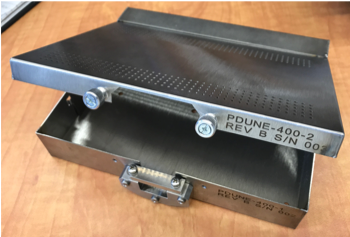
\includegraphics[width=0.45\linewidth]{tpcelec-box.png}
\end{dunefigure}
